\documentclass{jlcl}

%%%%%%%%%%%%%%%%%%%%%%%%%%%%%%%%%%%%%%%%%%%%%%%%%%%
%% information to be completed by the author(s): %%
%%%%%%%%%%%%%%%%%%%%%%%%%%%%%%%%%%%%%%%%%%%%%%%%%%%

%% Full author names, separated by commas
%\newcommand{\authornames}{INSERT FULL AUTHOR NAMES}
\newcommand{\authornames}{Author One and Author Two}


%% authors' last names, separated by commas
%\newcommand{\authorlastnames}{INSERT AUTHORS' LAST NAMES}
\newcommand{\authorlastnames}{One and Two}


%% Full article title, as it appears on the first page of the article
%\newcommand{\articletitle}{INSERT FULL ARTICLE TITLE}
\newcommand{\articletitle}{Internationalization}


%% short article title, as it appears in the header of every second article page
%\newcommand{\shortarticletitle}{INSERT SHORT ARTICLE TITLE}
\newcommand{\shortarticletitle}{Internationalization}


%% load babel package for the language the article is written in,
%% please refer to
%% http://tug.ctan.org/tex-archive/macros/latex/required/babel/babel.pdf
%% for other language options and add languages, if necessary
\usepackage[utf8]{inputenc}
\usepackage[LFE,LAE,T1]{fontenc}
%\usepackage[ngerman,english]{babel}     %% english & ngerman
\usepackage[ngerman, main=english]{babel} % arabic => problem with sections


% % % % % CUSTOM % % % % %
%%please add any packages your article needs which are not already included in the class
%\usepackage{}
\usepackage{ifxetex}


%=======Arabic=======
%% Contributions by Adrien Barbaresi, Kais Haddar, Osama Hamed.
\usepackage{arabtex}


% % % TODO: add Chinese to test Unicode support
\ifxetex
%\usepackage{xeCJK}
%\setCJKmainfont{SimSun}
\else
\usepackage{CJKutf8}
\fi


% % % Bibliography
\usepackage{apacite}


%%%%%%%%%%%%%%%%%%%%%%%%%%%%%%%%%%%%%%%%%%%%%%%%%%%%%%%
%% information to be completed by the typesetter(s): %%
%%%%%%%%%%%%%%%%%%%%%%%%%%%%%%%%%%%%%%%%%%%%%%%%%%%%%%%

\newcommand{\jlclvolume}{32}

\newcommand{\jlclnumber}{1}

\newcommand{\jlclyear}{2017}

\newcommand{\jlclfirstpage}{1}
%%==========================================================================================%%
%%==========================================================================================%%


\title{\articletitle}
\author{AUTHOR NAME\\
AUTHOR INSTITUTION\\
\texttt{AUTHOR EMAIL} \and
AUTHOR 2 NAME\\
AUTHOR 2 INSTITUTION\\
 \texttt{AUTHOR 2 EMAIL}}
 
%%==========================================================================================%%
\begin{document}

% arabtex
\setarab % choose the language specific conventions
\vocalize % switch diacritics for short vowels on
\transtrue % additionally switch on the transliteration
% \arabtrue % default


\setcounter{page}{1}
\thispagestyle{firstpage}

\authordata


%%==========================================================================================%%
%%           ARTICLE                                                                        %%
%%==========================================================================================%%

% to change language for babel package in the course of the article:
%\selectlanguage{english}

\section*{Abstract}
This article runs a series of tests to check internationalization and compatibility issues in the JLCL class.



\section{Arabic}

\subsection{The Alphabet}

%The Arabic alphabet has 29 letters including the Hamza (\textRL{ء}), consonants and three long vowels (\textAR{ا، و، ي}).
%The short vowels or vowel signs are not part of alphabet but they are merely oral.
%Along with the three short vowels (\textRL{ـَ ـُ ـِ}), the Arabic script has other phonetic symbols, together known as diacritic marks.
%Diacritics are sound symbols represented as strokes that are placed above or below the letter.

% % % solution found on http://tex.stackexchange.com/questions/141832/babel-arabic-changes-enumeration-level
This is a test: \RL{b.hr lw.t}

\begin{RLtext}'imtala'ati al-_dAkiraTu al-'iliktrUniyyaTu bi-mo`.tayAtiN `a^swA'iyyaTiN\end{RLtext}


\section{Chinese}

\subsection{Test}

\ifxetex
does not currently work with XeTeX.
%文章内容。 % % does not work
\else
\begin{CJK*}{UTF8}{gbsn}
文章内容。
%\clearpage
\end{CJK*}
\fi


\section{Figures}

\begin{figure}[h]
\centering
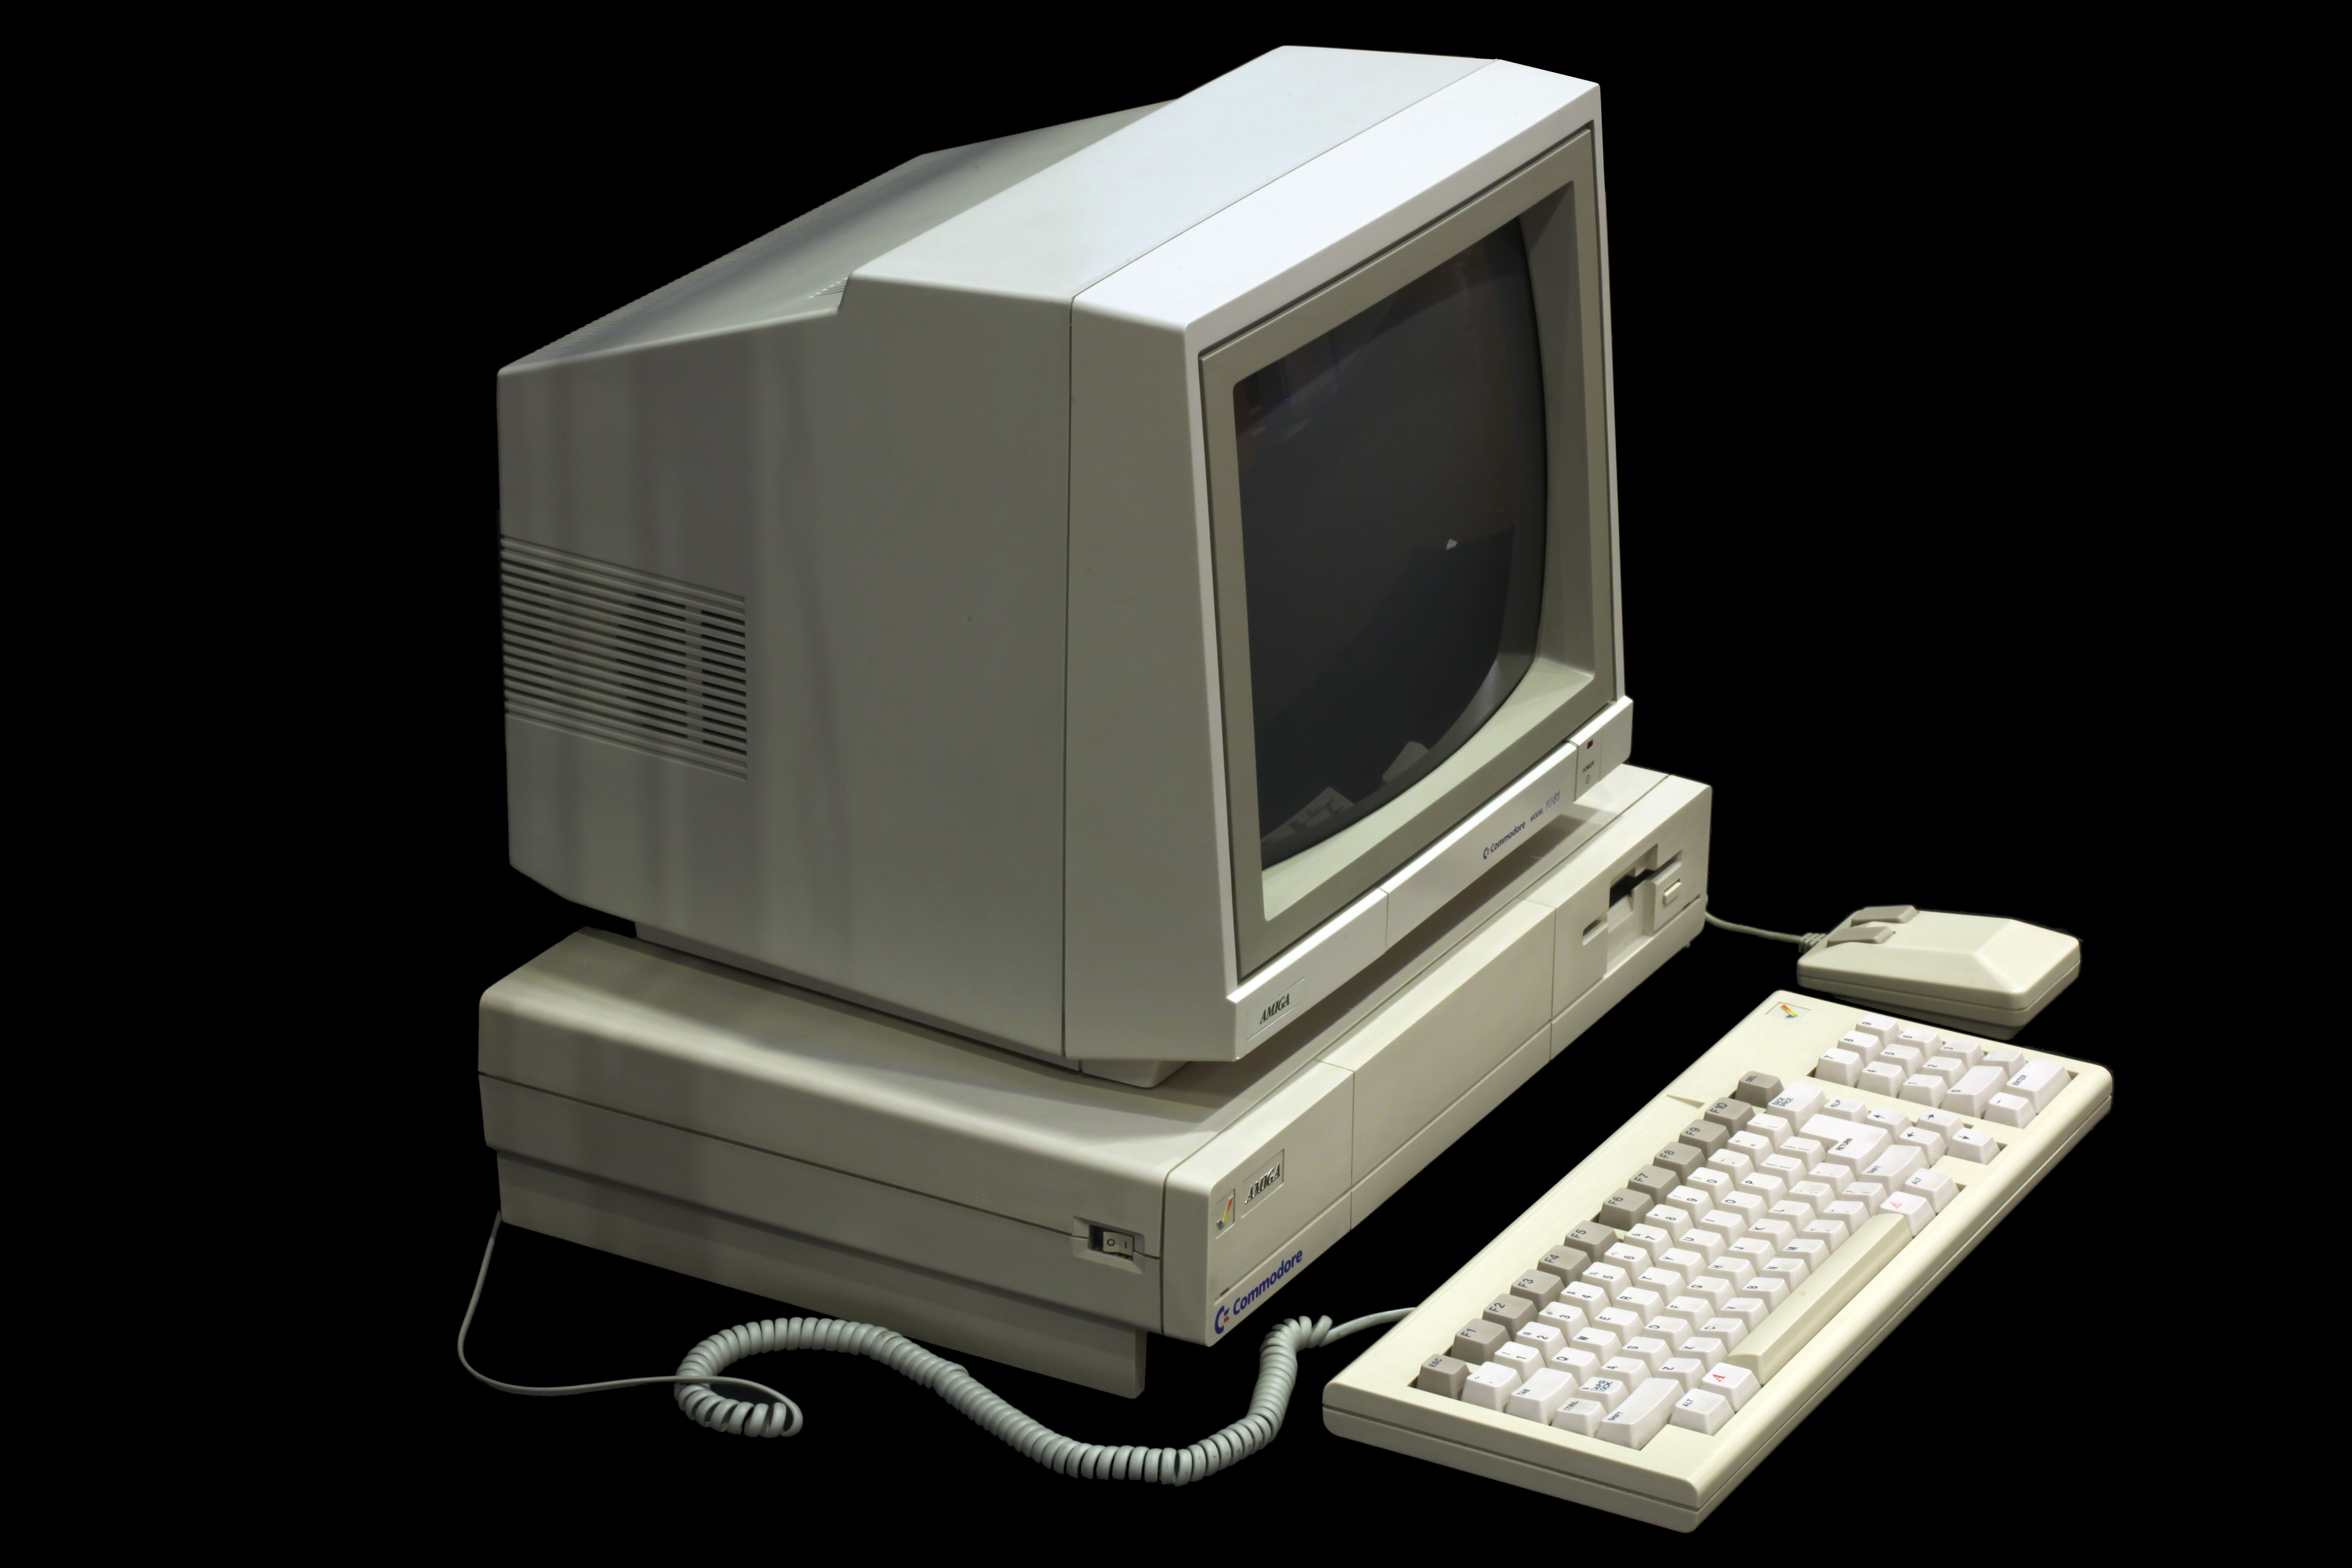
\includegraphics[width=0.7\textwidth]{Amiga_A1000.jpg}
\caption{Amiga A1000 on display at the Mus\'{e}e Bolo (Lausanne), Wikimedia user Rama \newline https://commons.wikimedia.org/wiki/File:Amiga\_A1000\_IMG\_4277.jpg}
\end{figure}



\nocite{*}
\bibliographystyle{apacite}
\bibliography{references}

%\printbibliography


\end{document}